% Internal draft figures only. Requires graphicx in the main preamble.
% Move individual environments to their corresponding paper sections.
% All paths are relative to the paper root; build from that directory.

\begin{figure*}[t]
  \centering
  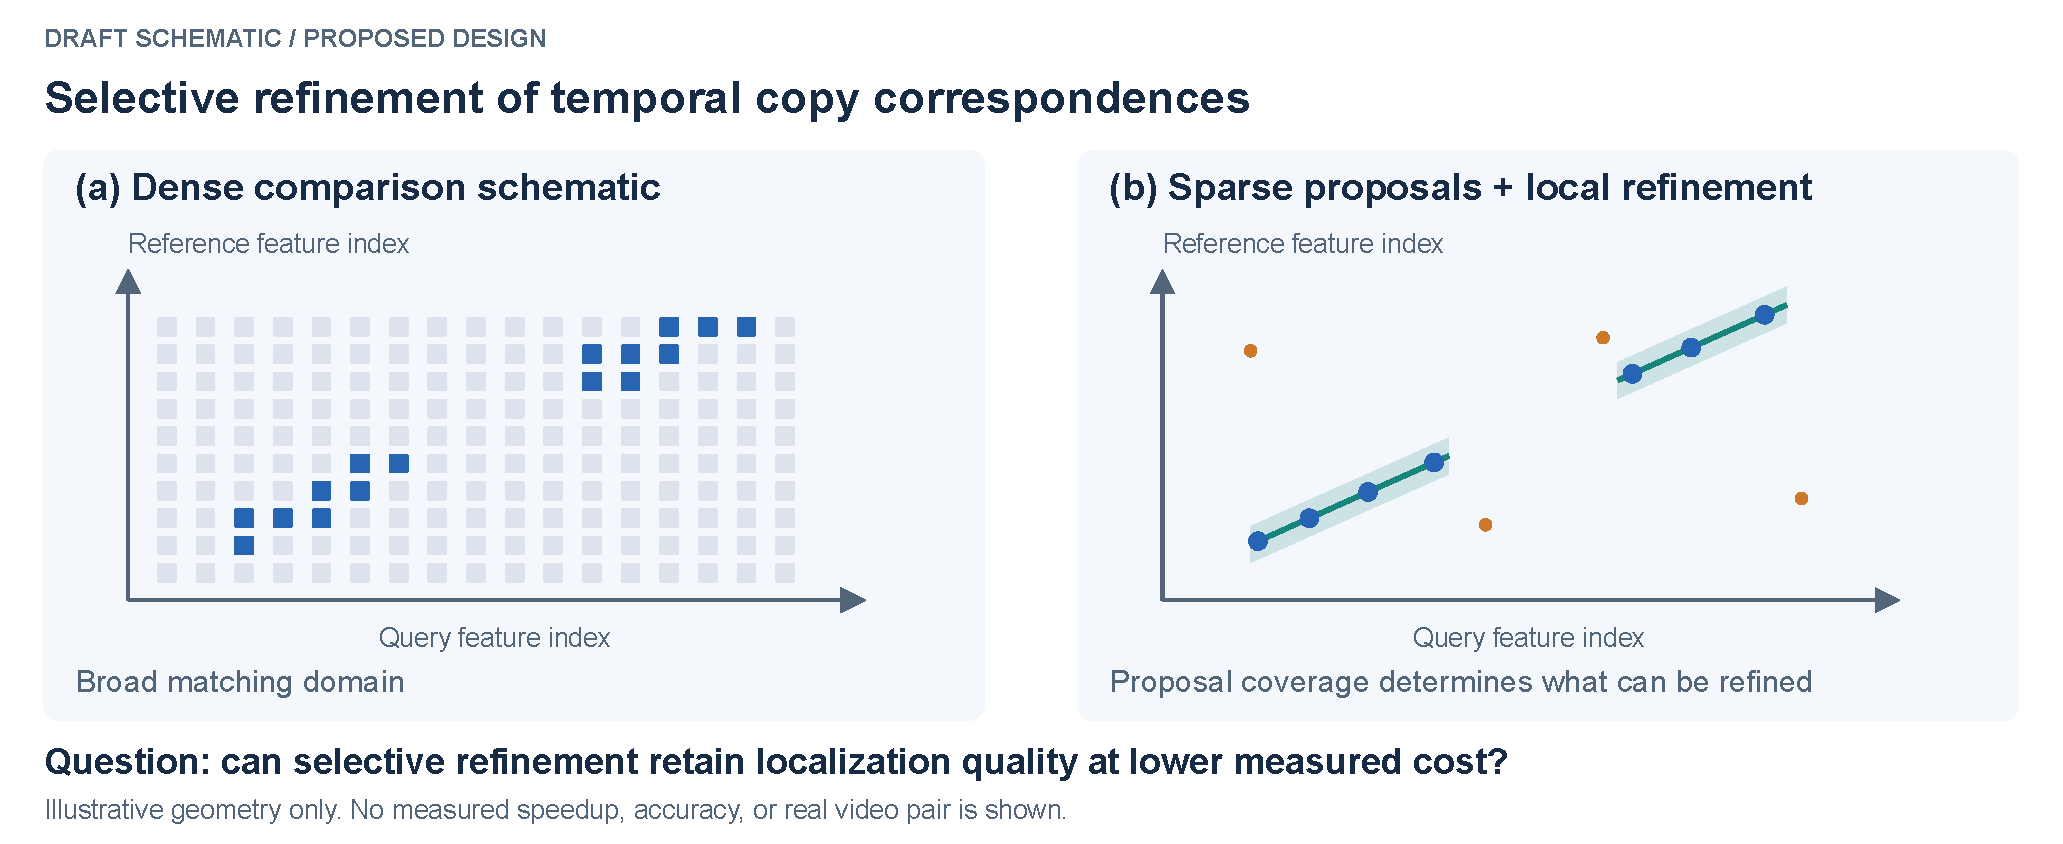
\includegraphics[width=\textwidth]{figures/fig_1_teaser.pdf}
  \caption{\textbf{Conceptual comparison of matching domains.}
  Dense comparison examines a broad frame-pair domain, whereas the proposed
  sparse-to-tube design uses temporal proposals to restrict fine-resolution
  alignment. The geometry is illustrative and does not represent a measured
  baseline or experimental output.}
  \label{fig:teaser}
\end{figure*}

\begin{figure*}[t]
  \centering
  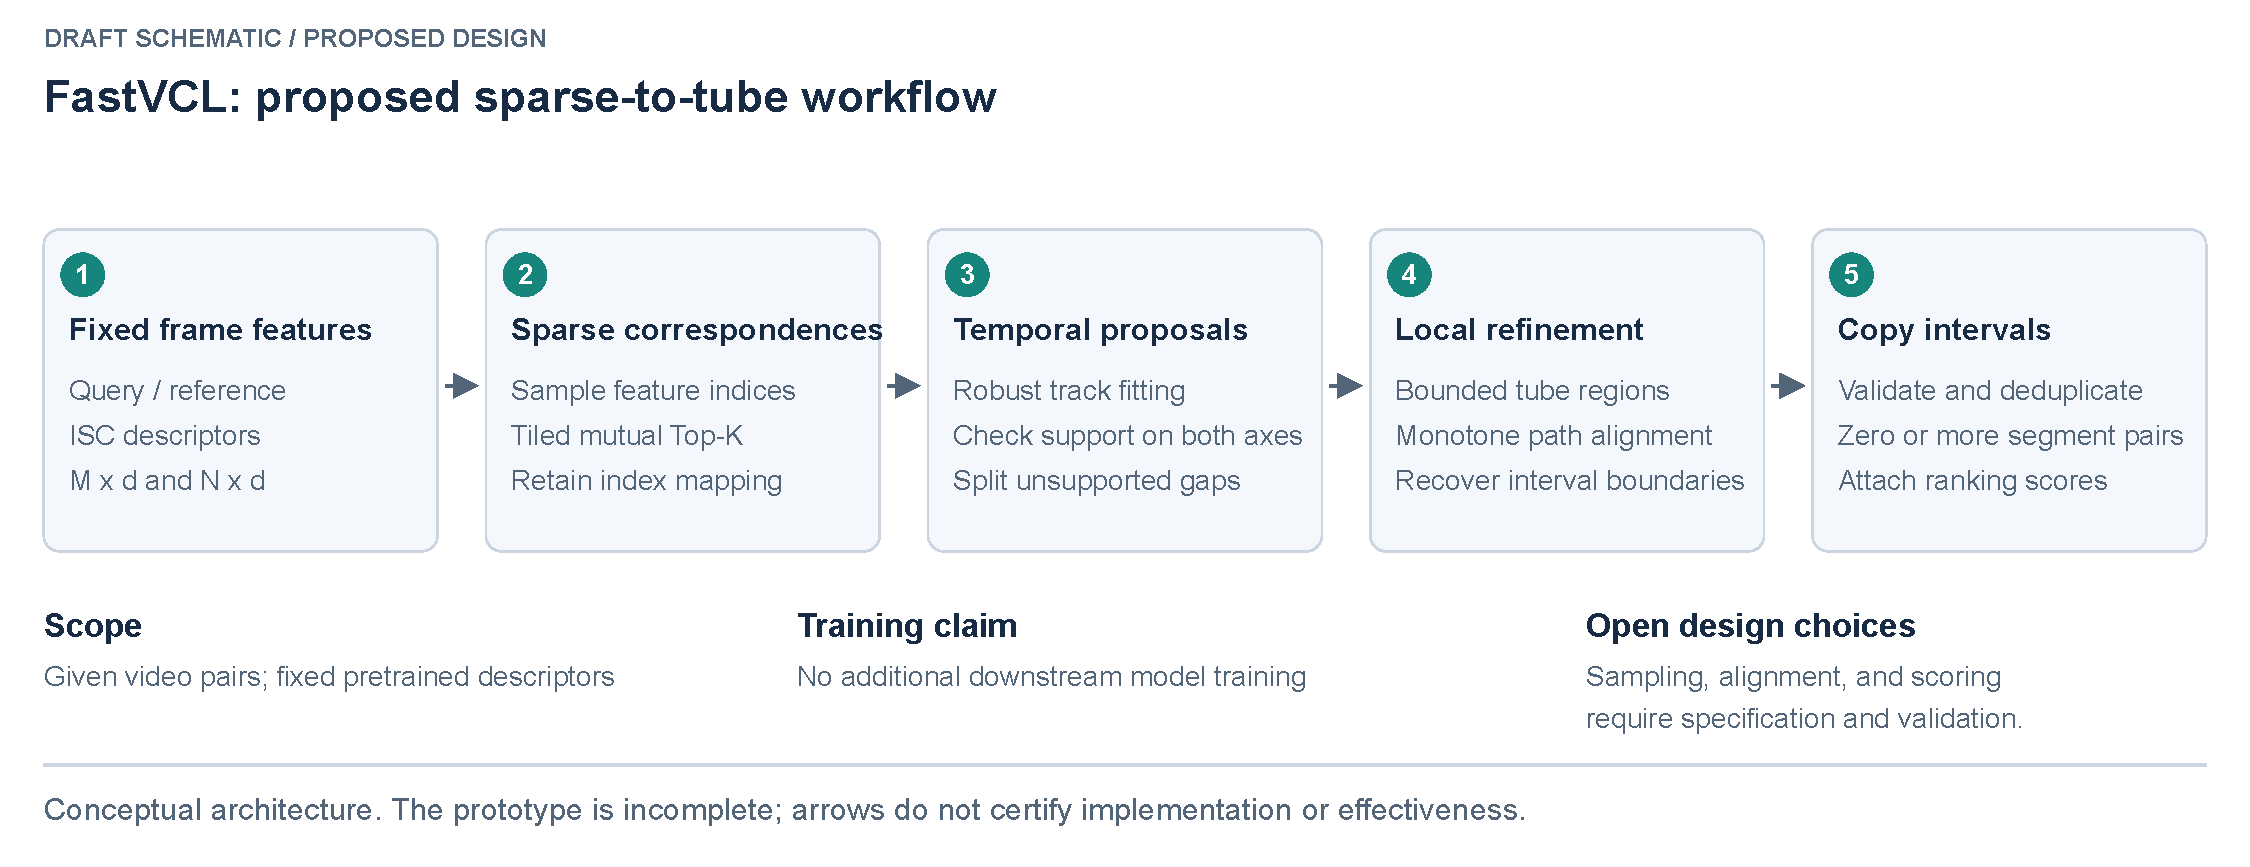
\includegraphics[width=\textwidth]{figures/fig_2_framework.pdf}
  \caption{\textbf{FastVCL framework (proposed method).}
  Fixed ISC descriptors are normalized, sampled and matched by tiled mutual
  Top-$K$. Coordinate-deduplicated anchors undergo RANSAC, dual-axis support checks
  and gap splitting to define finite tubes. The dashed blue connection reuses
  full-resolution descriptors for in-tube similarities. Proposed zero-floored
  local DP, backtrace, trimming, scoring and dual-axis de-duplication yield candidate
  intervals. One shared \texttt{seltive model} is queried at two budgeted insertion
  points: before fitting, to remove doubtful anchors ($A_0\to A_1$), and after
  extraction, to decide whether fragments are one continuous copy ($C_0\to Y$). Both
  read original A/B frames through a verified index map and abstain on uncertainty or
  failure; taking no action retains the core evidence. Backend, frame map and
  thresholds are not yet validated. Matrices and trajectories are schematic, not
  experimental outputs.}
  \label{fig:framework}
\end{figure*}

\begin{figure*}[t]
  \centering
  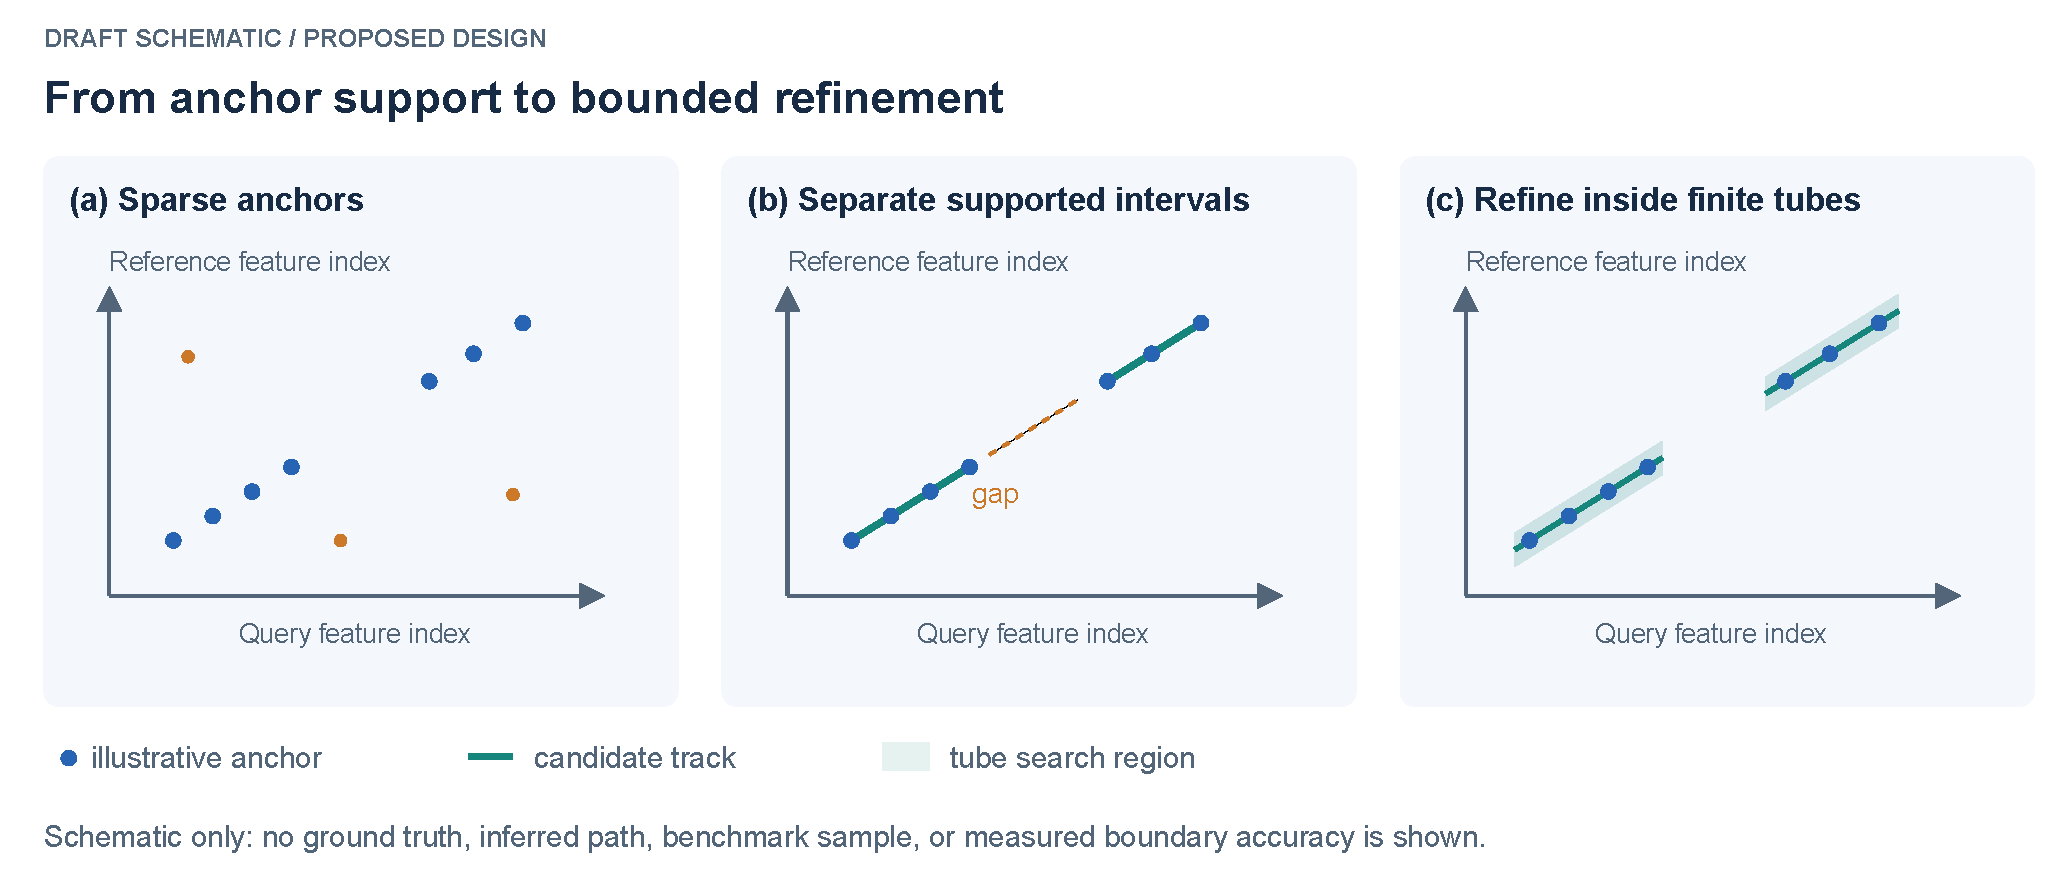
\includegraphics[width=\textwidth]{figures/fig_3_sparse_tracks.pdf}
  \caption{\textbf{Illustration of anchor-supported refinement.}
  Sparse correspondences suggest separated support intervals, which define finite
  tube regions for local alignment. All coordinates are schematic; this figure is
  not a qualitative benchmark result.}
  \label{fig:sparse_tracks}
\end{figure*}

\begin{figure*}[t]
  \centering
  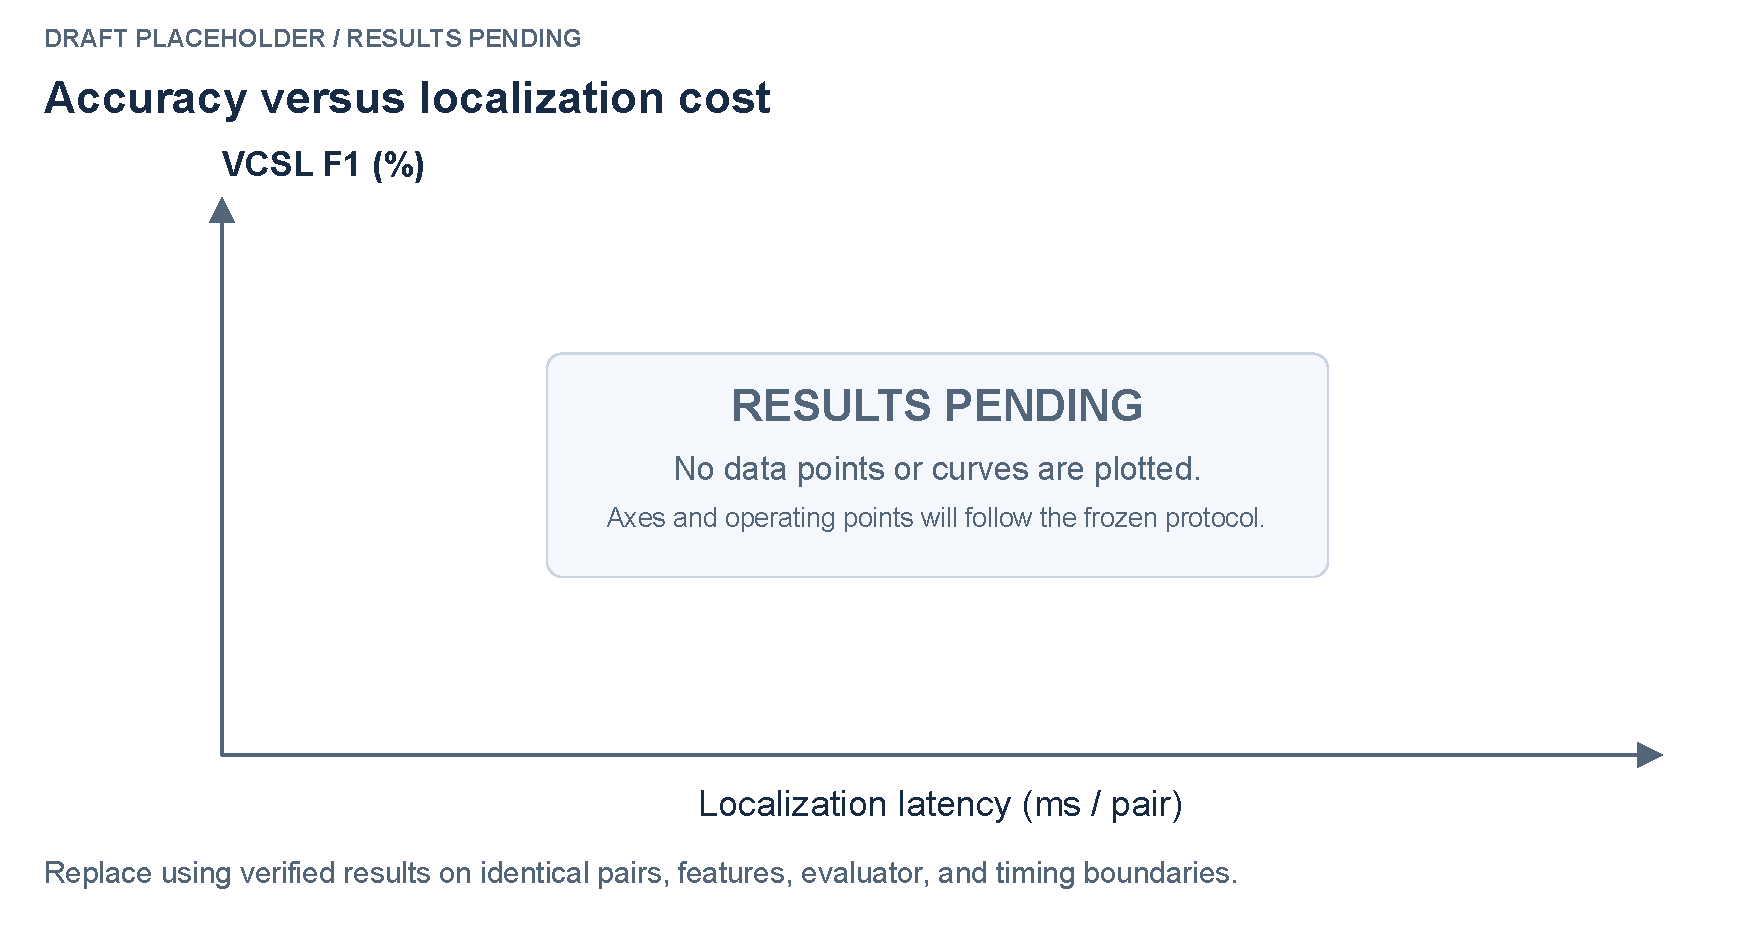
\includegraphics[width=\textwidth]{figures/fig_4_tradeoff.pdf}
  \caption{\textbf{Placeholder for the accuracy--latency comparison.}
  No measurements are shown. Operating points will be populated from verified
  runs using a frozen evaluation and timing protocol.}
  \label{fig:tradeoff}
\end{figure*}
